Controllable person image generation aims to generate a person image conditioned on reference images, allowing precise control over the person's appearance or pose.
However, prior methods often distort fine-grained details from the reference image, despite achieving high overall image quality.
We attribute these distortions to inadequate attention to corresponding regions in the reference image.
To address this, we thereby propose \textbf{learning flow fields in attention} (\textbf{\leffa{}}), which explicitly guides the target query to attend to the correct reference key in the attention layer during training.
Specifically, it is realized via a regularization loss on top of the attention map within a diffusion-based baseline.
Our extensive experiments show that \leffa{} achieves state-of-the-art performance in controlling appearance and pose, significantly reducing fine-grained detail distortion while maintaining high image quality.
Additionally, we show that our loss is model-agnostic and can be used to improve the performance of other diffusion models.

\begin{figure}[t]
\centering
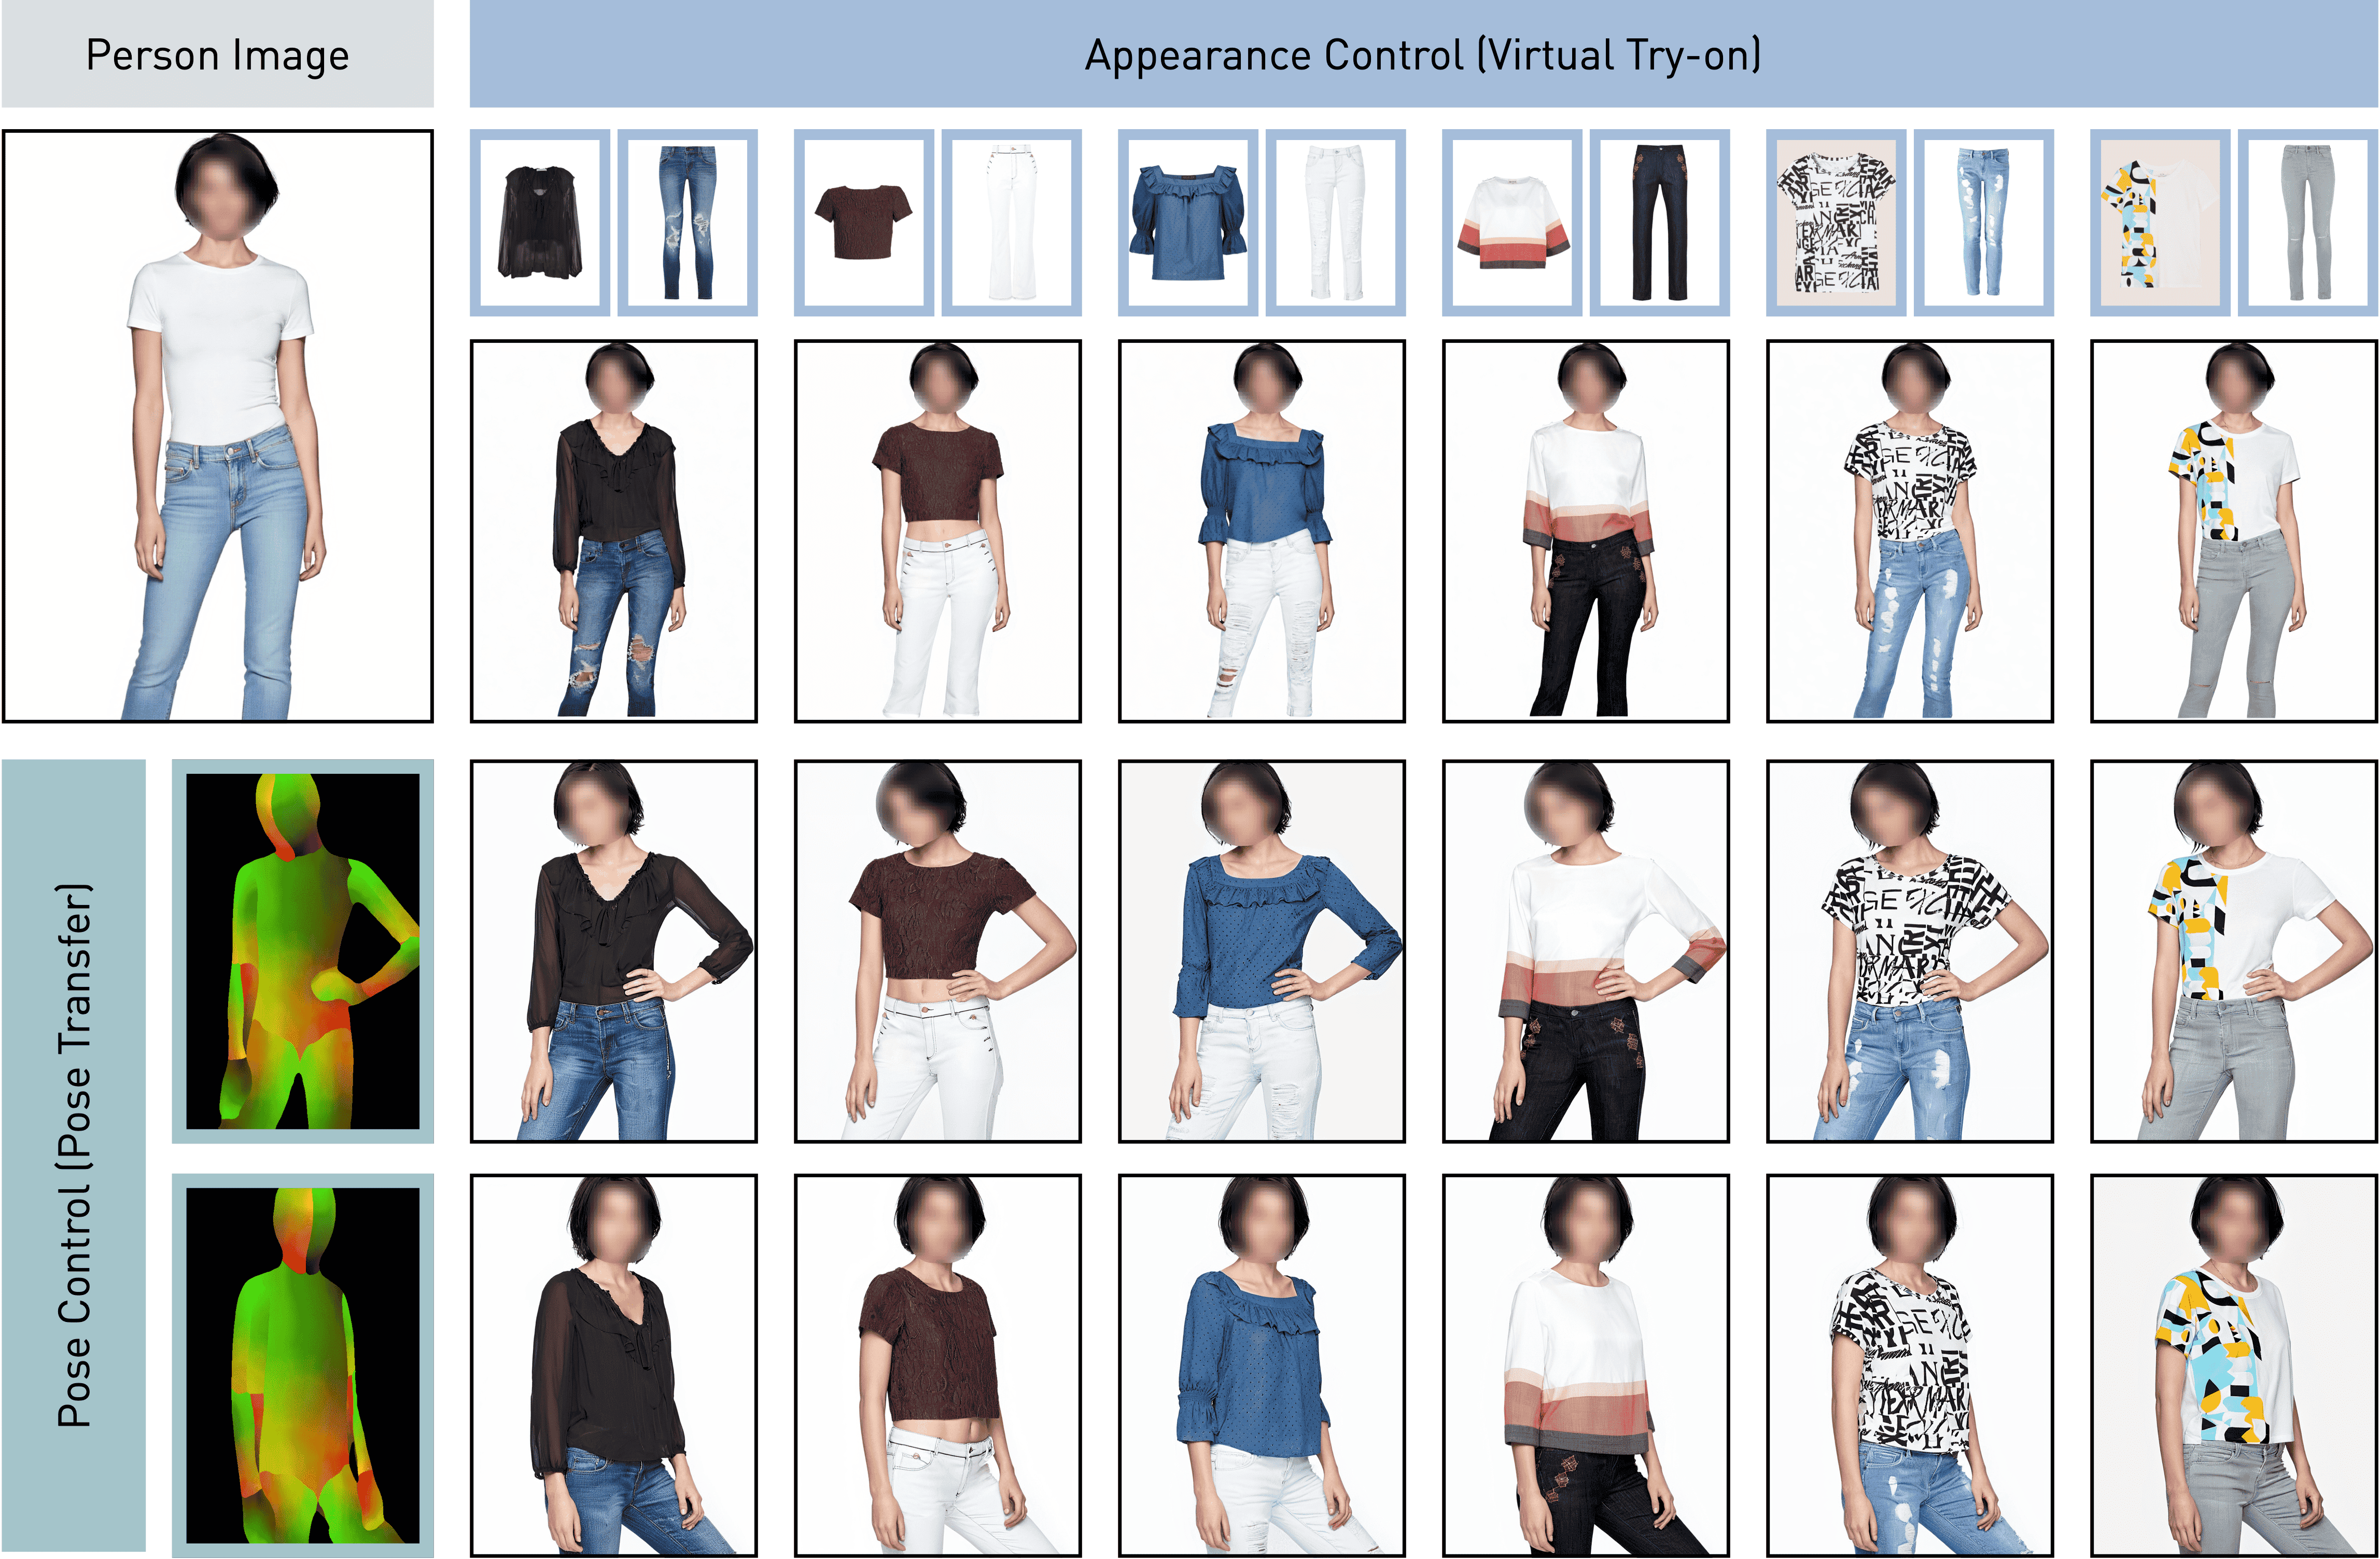
\includegraphics[width=\textwidth]{Chapter6/Figures/teaser_final-min.png}
\caption{
We present \leffa{}, a unified framework for controllable person image generation that enables precise manipulation of both appearance (\ie, virtual try-on) and pose (\ie, pose transfer). \leffa{}'s generated images demonstrate high quality, with fine details preserved and minimal texture distortion.
Please zoom in for better viewing.}
\label{leffa:fig:teaser}
\end{figure}
